\subsection{Phase III\label{sec:phaseIII}}

Phase I was about proving a concept and demonstrating that a less fragmented DeFi space was possible. Phase II was about enhancing and increasing the features of Mosaic as well as adding new liquidity models. Phase III is focused on increasing the decentralization of our solution. 

Mosaic’s core consists on a network of bridges, operated by relayers interacting with smart contracts on source and destination chain. Phase I and II are based on a trusted relayer solution, that monitors all connected chains for events, and enacts the transfers accordingly. Phase III improves on this model by decentralizing the relayer, using different cutting-edge technologies such as Threshold-Signature-Scheme (TSS). We allow users to directly participate and monitor in Mosaic's core functionality.

\subsubsection*{RelayerSet}
Each one of the bridges that constitutes Mosaic will be maintained by a group of decentralized and distributed relayers. This set of relayers will manage accounts and smart contracts on both the source and the destination chain. RelayerSets may form a multi-signature account, or use TSS to collectively manage a single private key. The relayers monitor the source chains for XCT requests, and based on the parameters and funds transferred, create the appropriate transactions on the destination chain.

\subsubsection*{RelayerSet Creation}
We’ve chosen to use RelayerSets instead of single relayer nodes to reduce the chance of fraudulent relayers, as well as reducing the stake required to participate as a relayer. In order to increase the security of the RelayerSets, and decrease the risk of a sybil attack, we assign relayers at random to different RelayerSets on-chain.

A user who wants to form part of a relayer group of a given size sends a transaction and initiates the registration. The transaction includes, the identification of the user, the stake he is providing and the size of the TSS he would like to form part of. Algorithm \ref{alg:register_TSS} contains the pseudo-code of the joining process.

    	\begin{algorithm}[H]
			\caption{Register TSS group}
			\begin{algorithmic}[1]
				\Require $t_r \gets \{Stake, msg.sender, size\}$
				\Require groups.  
				\Require needs.
				
				\If{$t_r.Stake < Required Stake$}
				    \State \Return Err
				\EndIf
				
				\If{needs[$t_r$.size] $<$ groups[$t_r$.size] \& $\forall g \in groups[t_r.size] : msg.sender \not \in g$} 
				    \State g $\gets sample(Hash(msg.sender || prev-block-hash))$ 
				    \If{g.size $+ 1=$ $t_r$.size}
				        \State PerformTSS();
				    \Else
				        \If{g.size $<$ $t_r$.size}
				        \State g.size++
				        \State g.append(msg.sender)
				        \State WaitForOthers();
				        \Else
				    	\State \Return Err
				    	\EndIf
				    \EndIf
				\Else
				\State \Return Err
				\EndIf
				\State \Return g
			\end{algorithmic}
			\label{alg:register_TSS}
		\end{algorithm}

\subsubsection*{Staking and Slashing}
In any form of distributed system in which free actors can take part, there is an open door to malicious and/or selfish behaviour. Because every randomly-generated imaginary entity likes money \cite{LightningNetwork}, we need to provide our protocol with a mechanism that punishes malicious actors, while at the same time incentives and rewards honest behaviour.

A stake amount is required to form a RelayerSet, and to individual relayers to join an already established set. The total stake by a RelayerSet sets the budget for their disputable transactions. For a RelayerSet to commit fraud, more than threshold relayers need to commit fraud. For security reasons we may require an elevated percentage of the relayers within a set to contribute in creating a transaction. 

Both TSS and multi-signatures can be used to construct fraud proofs showing which specific relayers colluded, which then leads to a slash of funds on the source chain side. Verification of these fraud proofs is very efficient, as we do not need to prove that a fraudulent transaction was included in the destination chain, only that the relayers signed a fraudulent transaction.

Transactions may be disputed by validators for a certain amount of blocks, we refer to this as the dispute window. As the protocol has Alice submit the transactions for the XCT, both the RelayerSet and Alice need to collude to commit fraud, making the total $slashable_{amount} = funds_{transfered} + relayer_{stake}$. This means that the $funds_{transfered}$ on the destination chain need to remain locked for the duration of the dispute window.

Although $slashable_{amount}$ cannot effectively be reduced; we can unlock the user’s funds earlier, by having liquidity providers stake the $funds_{transferred}$ portion of the slashable amount. An ensurer node operates similarly to a validator (it serve both roles), and observes valid XCTs. The XCT specifies that it wishes a faster unlock on the destination side, and the total fee it is willing to pay for the underlying stake. An ensurer node may then choose to provide the stake for the specified fee. As the insurer node can observe the mempool, source chain, and destination chain state, it is able to determine finality and take the risk that the smart contract cannot. Thus, we provide a faster unlock method to the final user and an opportunity to experienced validators with greater risk appetite to gain additional fees.  An insurer node might be prohibitively expensive for individual users to run. We will provide some way to allow users to provide their assets to a pool, without significant risk.

\subsubsection{Protocol}
We devote this section to give a general overview of how the protocol of Mosaic v3 will operate and how the new RelayerSets integrate on the ecosystem. We also introduce the most common procedures to raise and audit a disagreement during the dispute window.

Let Alice be a user who wishes to transfer an asset from chain Source to chain Destination through a chosen RelayerSet. This cross chain transfer (XCT) consists of a two smart contract interactions; the first on the source chain, which locks assets (XCT-lock), and the second which unlocks funds on the destination layer (XCT-unlock).

Alice initiates the transaction on the source chain, locking the funds in a time locked contract and storing the parameters of the proposed transaction,  then confirms it will relay the transaction by interacting with the contract, which permanently locks the funds. (The confirmation can be negotiated and signed off-chain to reduce gas fees for the relayer).

After XCT-lock has been confirmed, the RelayerSet sends Alice the XCT-unlock transaction, which she commits on the destination chain. Fig.~(\ref{fig:v3_protocol}) illustrates the complete process.

\begin{figure}[h]
    \centering
    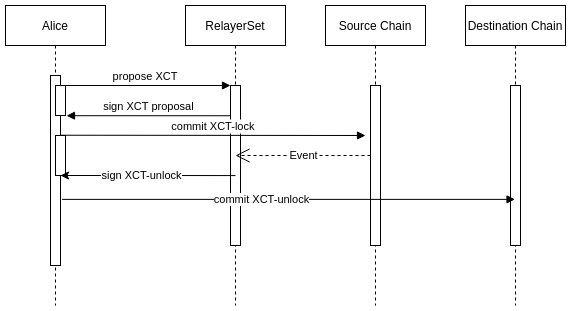
\includegraphics[width=0.75\textwidth]{images/mosaic/phase3/protocol.png}
    \caption{Time interaction scheme of the different actors for a XCT using RelayerSets. }
    \label{fig:v3_protocol}
\end{figure}

\subsubsection*{Disputes}
A malicious RelayerSet can commit fraud in a number of ways, which are handled through on-chain dispute and settled by slashing the stake of the relayers.

    \begin{itemize}
        \item \textbf{Case 1. RelayerSet and user submit a XCT-unlock with no corresponding XCT-lock on the source chain.}
        As illustrated in Fig.~(\ref{fig:dispute1}), when a validator observes a fraud on the destination chain, he musts dispute the RelayerSet on the source and destination chain. Disputes on the source chain are more easily settled since the validator only needs to submit the XCT-unlock event to show the intention of the relayer to commit fraud, independently of the inclusion or finality on the destination chain. 
        
        However, disputes on the destination chain are way more complex since different chains present different finality and consensus models. In order to address this problem, we resort to different proof-of-non-membership that can immediately settle the dispute. If that is not feasible, the dispute may be resolved through decentralized governance.
        
        \begin{figure}[h]
            \centering
            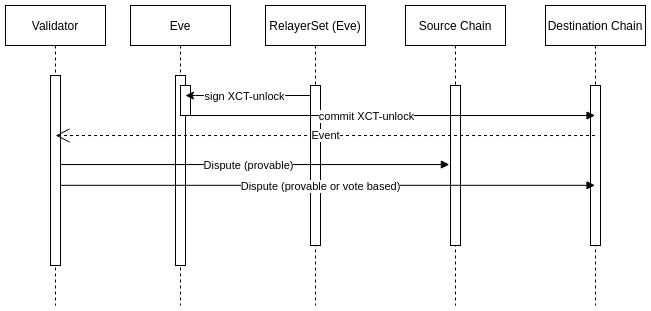
\includegraphics[width=0.75\textwidth]{images/mosaic/phase3/dispute1.png}
            \caption{Time interaction scheme of the dispute resolution when no XCT-lock event is triggered on source chain.}
            \label{fig:dispute1}
        \end{figure}
        
        
        \item \textbf{Case 2. RelayerSet and/or user create a transaction in the destination chain with a different corresponding transaction on source chain.}
        The solution to this dispute is actually identical to the previous one, as there will be no corresponding entry for the transaction on the source chain. Nonetheless, this case will be less common, as the amount of funds lost by the user is greater (the stake + the cost of the XCT-lock transaction), while it does not present additional gains with regards to case 1.
        
        \item \textbf{Case 3. RelayerSet does not create a corresponding transaction on destination chain.}
        Since the RelayerSet confirms on the source chain that it will relay by signing the XCT proposal, the fraud proof becomes showing the destination chain that RelayerSet committed to signing an XCT-unlock. The user can then re-obtain their funds on the destination chain. The proof is depicted in Fig.~(\ref{fig:dispute3}).
        
        \begin{figure}[h]
            \centering
            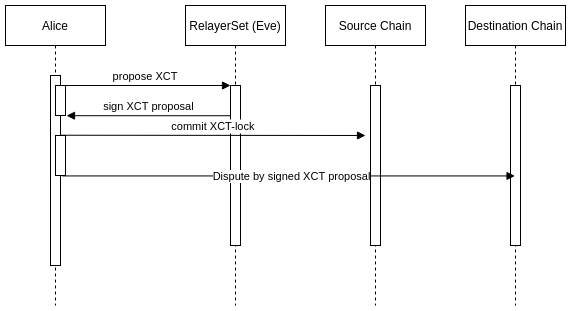
\includegraphics[width=0.75\textwidth]{images/mosaic/phase3/dispute3.png}
            \caption{Time interaction scheme of the dispute resolution when no transaction is created on destination chain. }
            \label{fig:dispute3}
        \end{figure}
        
        In the case where an honest RelayerSet provides XCT-unlock, but the user does not submit the transaction, the RelayerSet may still submit the XCT-unlock transaction during the dispute window and slash funds from the XCT.
        Not all destination chains may support smarts contracts. In that case; it must be possible to construct a proof of (non)-inclusion for the destination chain. The user then re-obtains their funds on the source chain.

    \end{itemize}


\subsubsection{TSS vs Multi-signatures}

In a decentralized and distributed environment, we need a mechanism that allows for verification, integrity and non-repudiability of messages. The most common tool for this goal is the use of digital signatures. Digital signatures are an instrument of public key cryptography \cite{Diffie1976NewCryptography} that allows for public verification. Multiple signatures schemes exist, most of them are based on the initial standard of DSA \cite{DSSStandard} and can be summarized as the following set of algorithms:

\begin{itemize}
    \item Key generation$(1^{\lambda}) \rightarrow (sk,pk)$. As the algorithm that takes as input a security parameter $\lambda$ and produces the signing key $sk$ and the public verification key $pk$.
    
    \item Signature$(m, sk) \rightarrow \sigma$. Which is the algorithm that takes a message $m$ and the signing key $sk$ to produce a signature $\sigma$.
    
    \item Verification$(pk,\sigma, m) \rightarrow 1/0$ As the verification algorithm that takes the message $m$ and the signature $\sigma$ and verifies them using the public key $pk$. It outputs a boolean with the result of the verification.
\end{itemize}

For our cross-chain solution, we consider two well-known and established schemes: multi-signatures and TSS. Both schemes serve our purpose of redistributing the responsibility among a set of parties, but there are some key differences we summarize here. 

\begin{itemize}
    \item \textbf{Multi-signature:} As the name suggest, it is a scheme that involves multiple signatures. To be considered valid, different parties need to sign the same content. It can be architectured in a threshold manner such that a minimum of signatures is required to be considered valid (e.g: 2-out-of-3). It produces as many signatures as the set of parties involved.
    
    \item \textbf{TSS:} Threshold Signature Schemes \cite{Gennaro2019FastSetup, Canetti2021UCAbortsb} are a special kind of signatures that allow to redistribute the responsibility between a set of parties. In a TSS, the secret key is not known by any party, each party has a partial secret key, and needs to collaborate with the a minimum subset of the parties (e.g: 3-out-of-5) in order to produce a valid signature. Only one single signature is produced and there is no difference on the signature produced or the verification process, when compared to traditional signatures.
\end{itemize}

Both approaches have its benefits and drawbacks. On the one hand, multi-signature is easier to implement since it is based on independent signatures and requires no additional setup. However, it produces multiple signatures, increasing the costs on the blockchain and the verification times, since each individual signature needs to be separately verified.

On the other hand, TSS  require quite a complicated setup, with multiple sub-protocols and the use of homomorphic cryptography \cite{Moore2014PracticalSurvey}. Nonetheless, the verification is simpler and faster than the multi-signature scheme. A simple scheme of both signatures protocols is depicted in Fig.~(\ref{fig:signatures}).

\begin{figure}[H]
    \centering
    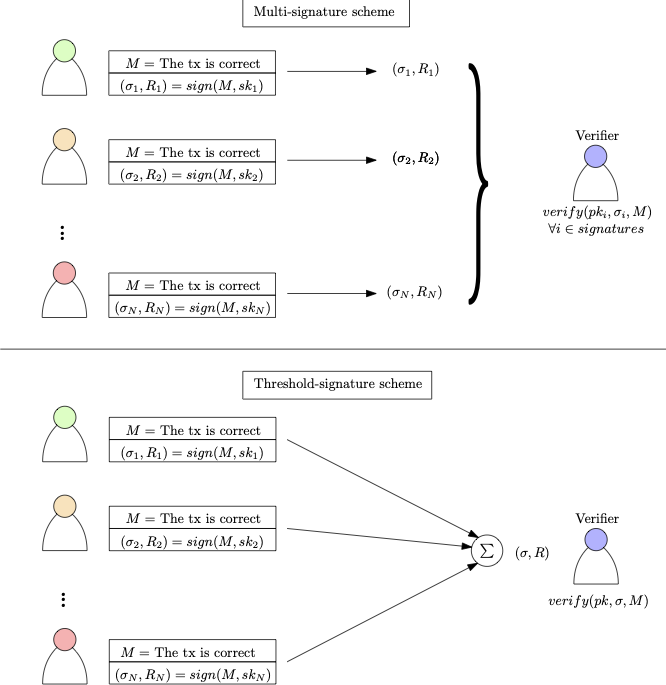
\includegraphics[width=0.9\textwidth]{images/mosaic/phase3/signatures.png}
    \caption{Multi-signature vs. TSS. Here, $\sigma$ represents a partial or complete signature, $R$ is the randomness used in the process, $M$ represents the message to be signed and $sk_i$ illustrates their partial or personal secret key.}
    \label{fig:signatures}
\end{figure}


Since we are focused an interested on keeping the operational costs as lower as possible for the user, we choose the TSS scheme. The setup can be performed off-chain, and then only a single signature and public verification key need to be broadcasted. This keeps the blockchain transaction and storage costs to a minimum while leveraging and state of the art signature scheme with all the desired security properties.


\subsubsection{Alternative model}
We presented the the protocol, the dispute resolution engine and the cryptographic constructs that enable Mosaic v3. However, there exist an alternative model we have also considered. In function of the data we gather from Phase II, we might consider this secondary approach. For the sake of completeness, we briefly describe the second model we considered.

As other projects have explored \cite{HopRollups, MOVRMOVR}, when a common layer or chain is available (e.g: L1 on Ethereum and RelayChain on Polkadot), cross-chain transfers can be achieved by bundling different transactions. The state (e.g: transactions or messages) from a source chain is transferred to the destination chain in a cryptographic accumulator, usually in the form of a Merkle Root \cite{Becker2008MerkleCryptanalysis}. As depicted in Fig.~( \ref{fig:accumulator}), the state is comprised on source chain and sent to the destination chain through the common layer. Later on, by proving membership  and unpacking the Merkle root, messages can be recovered on the destination layer.  By bundling information, we can reduce transaction costs on the common layer as well as benefiting from its security since the whole process is done on-chain. To ensure the validity of data being transferred, some stake is locked or an optimistic approach is pursued until the source chain settles its sates on the common chain. Then, the data is considered final and can be used as ground truth.

\begin{figure}[H]
    \centering
    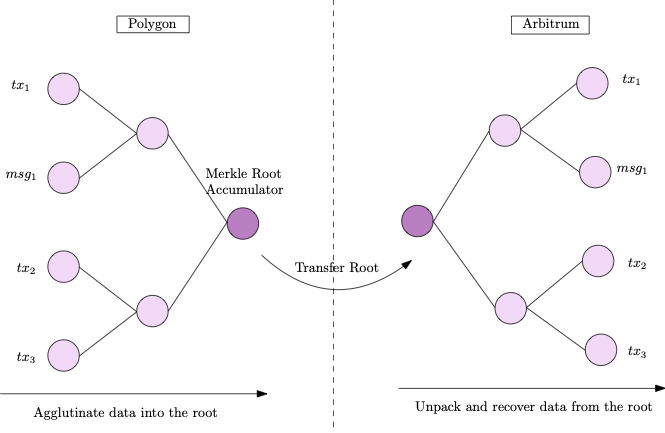
\includegraphics[width=0.9\textwidth]{images/mosaic/phase3/accumulator.png}
    \caption{Accumulate and transfer scheme. Only the Merkle root is transferred on-chain to  reduce costs.}
    \label{fig:accumulator}
\end{figure}

We believe Mosaic is more general than this approach, since it does not depend on the existence of a common layer and replaces the finality gadget with a set of decentralized relayers. Nonetheless, we might consider this agglutination scheme for scenarios in which a common layer can be easily found, in an effort to keep as much of the process on-chain. Please note that this approach still requires, to a certain degree, off-chain services in order to operate properly.